\documentclass[12pt, letterpaper]{article}
% must use this pkg for displaying imgs
\usepackage{graphicx}
\usepackage{amsmath}
\usepackage{multirow,array}
\usepackage{blindtext}
\usepackage{etoolbox}
\usepackage[a4paper, total={6in, 9in}]{geometry}
\graphicspath{ {../../imgs/} }
% pkg for links
\usepackage{hyperref}
% for codeblocks highlighting
\usepackage{color}
\usepackage{xcolor}
\usepackage{listings}

% Solarized colour scheme for listings
\definecolor{solarized@base03}{HTML}{002B36}
\definecolor{solarized@base02}{HTML}{073642}
\definecolor{solarized@base01}{HTML}{586e75}
\definecolor{solarized@base00}{HTML}{657b83}
\definecolor{solarized@base0}{HTML}{839496}
\definecolor{solarized@base1}{HTML}{93a1a1}
\definecolor{solarized@base2}{HTML}{EEE8D5}
\definecolor{solarized@base3}{HTML}{FDF6E3}
\definecolor{solarized@yellow}{HTML}{B58900}
\definecolor{solarized@orange}{HTML}{CB4B16}
\definecolor{solarized@red}{HTML}{DC322F}
\definecolor{solarized@magenta}{HTML}{D33682}
\definecolor{solarized@violet}{HTML}{6C71C4}
\definecolor{solarized@blue}{HTML}{268BD2}
\definecolor{solarized@cyan}{HTML}{2AA198}
\definecolor{solarized@green}{HTML}{859900}
\definecolor{solarized@orchid}{HTML}{483D8B}


% Define C++ syntax highlighting colour scheme
\definecolor{commentgreen}{RGB}{2,112,10}
\definecolor{eminence}{RGB}{108,48,130}
\definecolor{weborange}{RGB}{255,165,0}
\definecolor{frenchplum}{RGB}{129,20,83}

\lstset {
    language=[GNU]C++,
    frame=tb,
    tabsize=4,
    showstringspaces=false,
    numbers=left,
    upquote=true,
    commentstyle=\color{commentgreen},
    keywordstyle=\color{solarized@orchid},
    identifierstyle=\color{solarized@blue},
    stringstyle=\color{solarized@magenta},
    basicstyle=\small\ttfamily, % basic font setting
    emph={int,char,double,float,unsigned,void,bool},
    emphstyle={\color{blue}},
    escapechar=\&,
    % keyword highlighting
    classoffset=1, % starting new class
    otherkeywords={TEST, EXPECT_EQ,>,<,.,;,-,!,=,~, typename},
    morekeywords={TEST, EXPECT_EQ,>,<,.,;,-,!,=,~, typename},
    keywordstyle=\color{frenchplum},
    classoffset=0
}

\makeatletter
\patchcmd{\raggedright}{\parindent\z@}{}{}{}
\makeatother

\begin{document}


\newcommand{\paperauthor}{Akiel Aries}
\newcommand{\papersupervisor}{Prof. Sareh Assiri}
\newcommand{\paperuniversity}{Northern Arizona University}

\newcommand{\papertitle}{Analyzing and Reporting on}
\newcommand{\paperminortitle}{Stuxnet}
\newcommand{\papermajorheading}{Cybersecurity}
\newcommand{\paperminorheading}{CYB 410 - Software Security}

\newcommand{\HRule}{\rule{\linewidth}{0.5mm}} % Defines a new command for the horizontal lines, change thickness here

\center % Center everything on the page

%----------------------------------------------------------------------------------------
%	HEADING SECTIONS
%----------------------------------------------------------------------------------------

\textsc{\LARGE \paperuniversity}\\[1.0cm] % Name of your university/college
\textsc{\Large \papermajorheading}\\[0.2cm] % Major heading such as course name
\textsc{\large \paperminorheading}\\[0.75cm] % Minor heading such as course title

%----------------------------------------------------------------------------------------
%	TITLE SECTION
%----------------------------------------------------------------------------------------

\HRule \\[0.4cm]
{ \huge \bfseries \papertitle}\\[0.05cm] % Title of your document
{ \huge \paperminortitle}\\[0.025cm] % Title of your document
\HRule \\[3.5cm]

\begin{center}
	\makebox[1.0\textwidth]{
\includegraphics[width=1.0\textwidth]{stuxnet.jpg}}
\end{center}


\vfill % Fill the rest of the page with whitespace
%----------------------------------------------------------------------------------------
%	AUTHOR SECTION
%--------------------------------------------------------------------------------------

\begin{minipage}{0.4\textwidth}
	\begin{flushleft} \large
	\emph{Author:}\\
	\paperauthor
	\end{flushleft}
	\end{minipage}
	~
	\begin{minipage}{0.4\textwidth}
	\begin{flushright} \large
	\emph{Professor:} \\
	\papersupervisor
	\end{flushright}
\end{minipage}\\[1cm]

%----------------------------------------------------------------------------------------
%	DATE SECTION
%----------------------------------------------------------------------------------------
{\large \today}\\ % Date, change the \today to a set date if you want to be precise

\newpage

\begin{sloppypar}


% classification img
%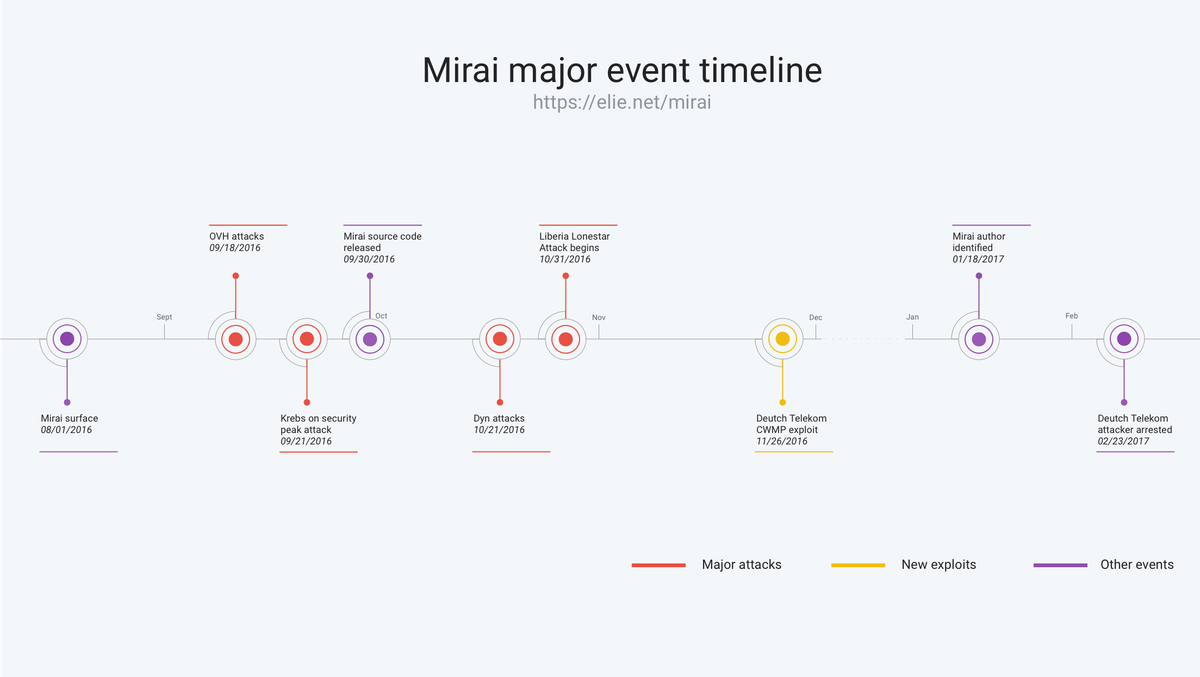
\includegraphics[scale=0.3]{mirai-major-events-timeline.png}
\begin{flushleft}
\section{Overview}
\begin{center}
{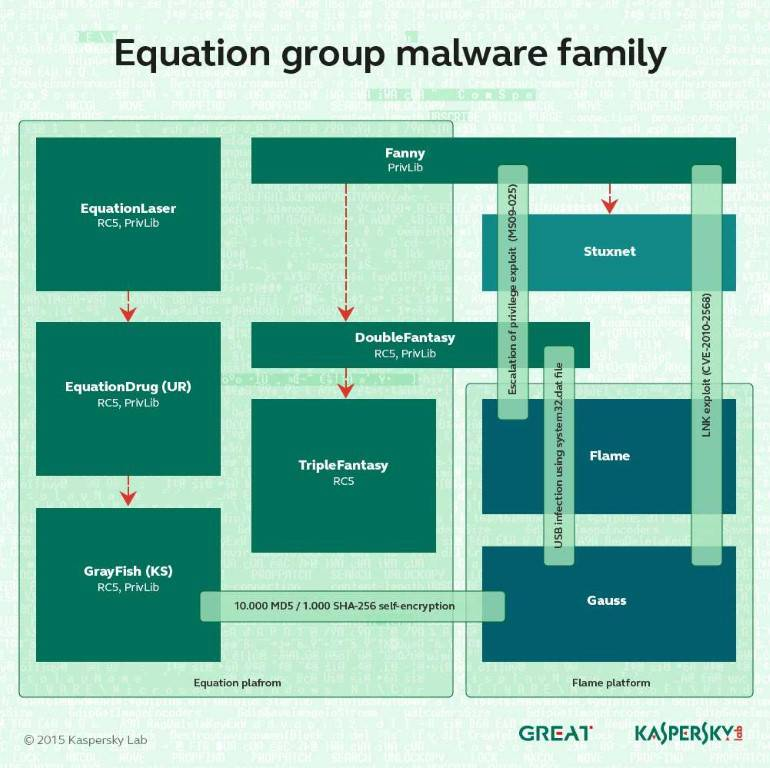
\includegraphics[width=0.9\textwidth]{equation_group_family.jpg}}
\end{center}
Stuxnet is a computer worm first identified in 2010 that was originally
implemented to target Iranian governments nuclear facilities. Just like 
most virus', they mutate and spawn new strains often more dangerous than
their predecessor. The original infection succeeded in targeting PLCs
(Programmable Logic Controller) which are used in a plethora of 
manufacturing related processes. For example, PLCs are used in robotic
machinery seen in assembly lines at manufacturing plants. The point of 
these controllers is to be secure, reliable, and useful fault diagnostics. 

It is no wonder why Stuxnet was a 
large threat in the InfoSec industry. It is of popular belief that this is
the first computer worm capable of affecting hardware and its peripherals as
most computer worms are built as software exploits. The origin of the worm is 
cloudy however, according to reports from cybersecurity research firms such 
as Kapersky Lab, Symantec, and many more, the origin supposedly started as 
a nation-based collaboration with the United States and Isreal to target the
Iranian Nuculear Program. The worm went on to destroy 1/5 of Iran's nuclear 
centrifuges, an important component in the process of enriching collected
uranium, infecting above 200,000 thousand devices and went on to severely 
degrade the performance of over 1,000 machines themselves. What lead 
researchers to believe the bug was nation state sponsored was the lack of
infections of other users of the Seimens based software. This was false 
according toe Eugene Kapersky himself as he said a Russian neuclear power
plant was also infected but not affected since it lacked any access to the
public-facing internet. The common belief is that the group behind the attack
is a nation state sponsored team by the name of Equation Group with reported
ties to the USA's National Security Agency (NSA) which is also believed to 
be a part of over 500 computer infections. When it comes to violation of the 
CIA triad, this becomes somewhat murky territory as the attack was supposedly
carried out the very own United States Government and the infected party was
exploited by means of an air gap, meaning the bot's initial attack vector
is physical. At a glance, all aspects of the CIA triad were violated as 
the confidentiality of the attack was not contained per leaked documents 
along with whistleblowing (allegedly), integrity was not upheld by the nation
or said party involved, and availability was not present.


The repository that this report will be base the code off of is located 
here: https://github.com/research-virus/stuxnet



%\newpage

\section{Fuzzing}
The stuxnet virus makes use of infecting RPC (Remote procedure call) servers based on 
the different type of call types that are made. The servers are split into two 
components one managing local RPC calls and the other for managing remote calls. 
The calls that were sniffed were services.exe for local calls.

The bot makes use of exploited Windows systems on a very low level allowing the attacker
to maniuplate portions of the Operating System perhaps not meant to be dealt with by 
regular users. Stuxnet makes effective use of exploiting at the time Windows inseucre 
digital certificate services. Stuxnet makes use of exploiting asynchronous encryption
methods utilized by said certificate services, this allows Stuxnet to infect and spread by
spawning processes different threads. To look into this I had found an example of simple
asynchronous encryption in C++, allowing for decription from the CLI as well. See here:
https://github.com/galets/oneway-cpp

When Fuzzing the program I had attempted for many hours to install deepstate produced
by trailofbits, but failed in every way including within a Docker container. To make use
of fuzzing the \verb|async_encrypt.cpp| file I made use of AFL and AFL++. Using AFL++ and getting 
it installed was quite the process but since my reinterpretation of an asynchronous 
encryption algorithm accepted argc and argv paramaters I had to do some research on how
this could be done. I went ahead and found a header file I could easily use along with
some macros to initialize argv fuzzing with the default argv[0] set to the compiled binary
itself. 
 
Fuzzing the code itself took some work. I had created a Makefile for easier compiliation
with the following contents:
\begin{verbatim}
oneway-AFL-COMP: 
	AFL_SKIP_CPUFREQ=1 AFL_HARDEN=1 afl-g++ -o \
	oneway_AFL oneway.cpp -lssl -lcrypto

oneway-AFL-RUN:
	AFL_SKIP_CPUFREQ=1 afl-fuzz -i in -o out ./oneway_AFL
\end{verbatim}
the \verb|AFL_SKIP_CPUFREQ| initializer skips the error that may pop up of innefecient 
CPU cycles. I chose to ignore this since the program I am testing is not large and I do
indeed have suffecient CPU cycles. Compiling the code with afl-g++ allows for us to 
compile the code with instrumentation to be recognized by the fuzzer itself. To fuzz the
code itself I had created an \verb|in/| directory with test inputs to fuzz against (mainly
just test cases of generating hashes in a asynchronous way) and generates an \verb|out|
directory with result of our fuzzer. This can be ran indefinitely and we can monitor the 
result as it goes. Here is an example of AFL++ running for about 25 minutes with the 
following results:

{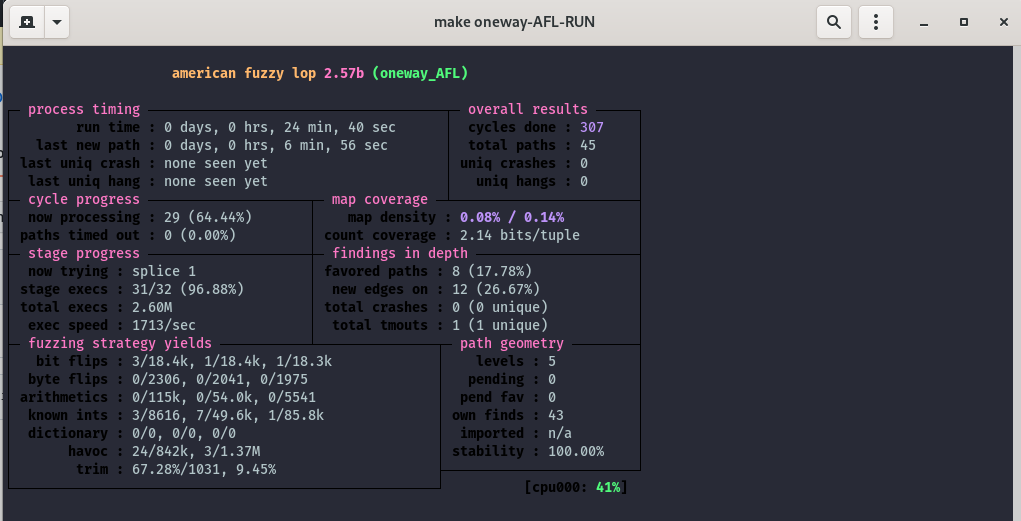
\includegraphics[width=1\textwidth]{AFL_test0.jpg}}

A number of 1 unique timeout was produced really being the only significant result. Perhaps
if I refactored the code (if it wasn't over 600 lines) with more time I could've produced
more interesting result but programs that make use of properly implemented CLI arguments
and flags are hard to fuzz against. 

%\newpage

\end{flushleft}
\end{sloppypar}
\end{document}
